\documentclass[11pt,a4paper]{article}
\usepackage[margin=22mm]{geometry}
\usepackage{amsmath,booktabs,graphicx,siunitx,hyperref}
\title{NAUSICAA: discharge correction calibrated from the CSA}
\author{Numerical study}\date{\today}
\begin{document}\maketitle
\section{Calibration}
The final 180 nm CSA uses M3 with $W=\SI{200}{\micro\metre}$,
$L=\SI{2}{\micro\metre}$ and gate bias \SI{0.538477478921}{V};
M4 has $W=\SI{2.88}{\micro\metre}$, $L=\SI{1.44}{\micro\metre}$
and gate bias \SI{0.556803417206}{V}. The external input capacitance is
\SI{1.25}{pF}, the feedback capacitor is \SI{3}{fF}, the supply is
\SI{1.8}{V}, and the temperature is \SI{20}{\celsius}. The supplied
NOIMOD=2 model includes intrinsic MOS capacitances and transistor noise.

The input is the finite-gap current for uniform ion collection over
\SI{20}{ms}. The benchmark is a central trajectory at \SI{3}{m/s} through
a \SI{5}{mm} gap to a square pad of side \SI{0.5}{mm} in an infinite grounded
plane. The gas is a homogeneous half-space. The weighting potential is one
on the pad, zero on the surrounding plane and tends to zero at infinity.
The integral per ion remains $e[1-\phi_w(g)]$.

After collection ends, the input current is zero and the CSA signal decays.
A matched zero-input run supplies the baseline. We fit the output change
from a 100-ion packet between 21 and 120 ms with
\[
 V(t)=B\exp[-(t-t_*)/\tau_0].
\]
The fit is linear in $\log[-V(t)]$, evaluated on a uniform \SI{200}{\micro\second}
grid, with free amplitude $B$. The fit starts \SI{1}{ms} after the last ion
is collected. It gives
\[
 \tau_0=\SI{2.454158}{s},\qquad
 \alpha=\exp[-\SI{20}{ms}/\tau_0]=0.99188368.
\]
The fitted time describes the decay of the complete CSA response. It includes
the transistor feedback path and the finite amplifier response.

The maximum relative fit residual is \num{3.7e-08}. A 10-ion calibration
changes the fitted time by a relative \num{5.82e-05}; halving the numerical
step changes it by \num{3.86e-06}. Fits to separate parts of the tail give:
\begin{center}\begin{tabular}{rrr}\toprule
Fit interval (ms) & $\tau_0$ (s) & Recalculated ENC\\\midrule
21--40 & 2.454139 & 112.70113 \\
40--80 & 2.454166 & 112.70114 \\
80--120 & 2.454156 & 112.70114 \\
\bottomrule\end{tabular}\end{center}
The fitted times over the tested 10--2000 ion range lie between
\SI{2.454105}{s} and \SI{2.454301}{s}.

\section{Readout and noise}
The readings are centred averages over \SI{300}{\micro\second}. The
measurement and calibrated ion estimate are
\[
 D_n=-[\overline V_n-\alpha\overline V_{n-1}],\qquad
 \widehat N_n=D_n/g.
\]
Both the gain $g$ and the noise are recalculated with the new $\alpha$.
The gain is obtained from the uniform mean response per ion. The same saved
stationary noise spectrum of the final circuit is integrated from
\SI{0.1}{Hz} to \SI{1}{MHz} with the averaging and difference filter:
\[
 \sigma_D^2=\int S_V(f)\operatorname{sinc}^2(fT_a)
 \left[(1-\alpha)^2+4\alpha\sin^2(\pi f\Delta t)\right]\,\mathrm{d}f,
 \qquad \mathrm{ENC}=\sigma_D/g.
\]
Here $\operatorname{sinc}(x)=\sin(\pi x)/(\pi x)$.

\begin{center}\begin{tabular}{lrr}\toprule
Quantity & Previous correction & Calibrated correction\\\midrule
Correction time (s) & 0.3000 & 2.4542 \\
$\alpha$ & 0.935507 & 0.991884 \\
Gain ($\mu$V/ion) & 27.127 & 27.119 \\
Noise in voltage difference (mV) & 3.042 & 3.056 \\
ENC (elementary charges RMS) & 112.14 & 112.70 \\
Previous-packet residual (\%) & 5.747 & 0.082 \\
Following-packet contribution (\%) & 0.517 & 0.518 \\
Minimum ions for $S/N>5$ & 562 & 564 \\
\bottomrule\end{tabular}\end{center}
The previous-packet entry is the signal in the first empty bucket following
an isolated packet, divided by its signal in its own bucket. The following-packet
entry arises from induction before collection and averaging across the boundary.
The correction removes most of the previous-packet contribution. The remaining
boundary response is included in the multi-bucket test below.

Direct finite-charge LTspice transients bracket the new threshold:
\begin{center}\begin{tabular}{rr}\toprule
Ions & $S/N$\\\midrule
563 & 4.992068 \\
564 & 5.000928 \\
\bottomrule\end{tabular}\end{center}
The noise is stationary about the quiescent operating point. Signal amplitudes
come from the nonlinear transistor transients.

\section{Consecutive and empty buckets}
An independent transient contains the following sequence of uniform packets.
Each estimate uses the same gain and correction calibrated above.
\begin{center}\begin{tabular}{rrrr}\toprule
Bucket & Input ions & Previous estimate & Calibrated estimate\\\midrule
1 & 1000 & 1003.94 & 1003.94 \\
2 & 1000 & 1053.72 & 997.14 \\
3 & 0 & 116.00 & 3.39 \\
4 & 500 & 608.99 & 497.25 \\
5 & 0 & 149.70 & 10.70 \\
6 & 2000 & 2125.67 & 1987.77 \\
7 & 1000 & 1238.06 & 988.96 \\
8 & 0 & 303.92 & 0.82 \\
\bottomrule\end{tabular}\end{center}
The largest absolute error changes from 303.92 to 12.23 ions over this
sequence, compared with an ENC of 112.70 elementary charges RMS. These
estimates use the deterministic waveforms; random noise has not been added
to the displayed sequence. The noise level is calculated separately from
the output spectrum. The test establishes the accuracy over this sequence
of charge levels and arrival times.

\begin{center}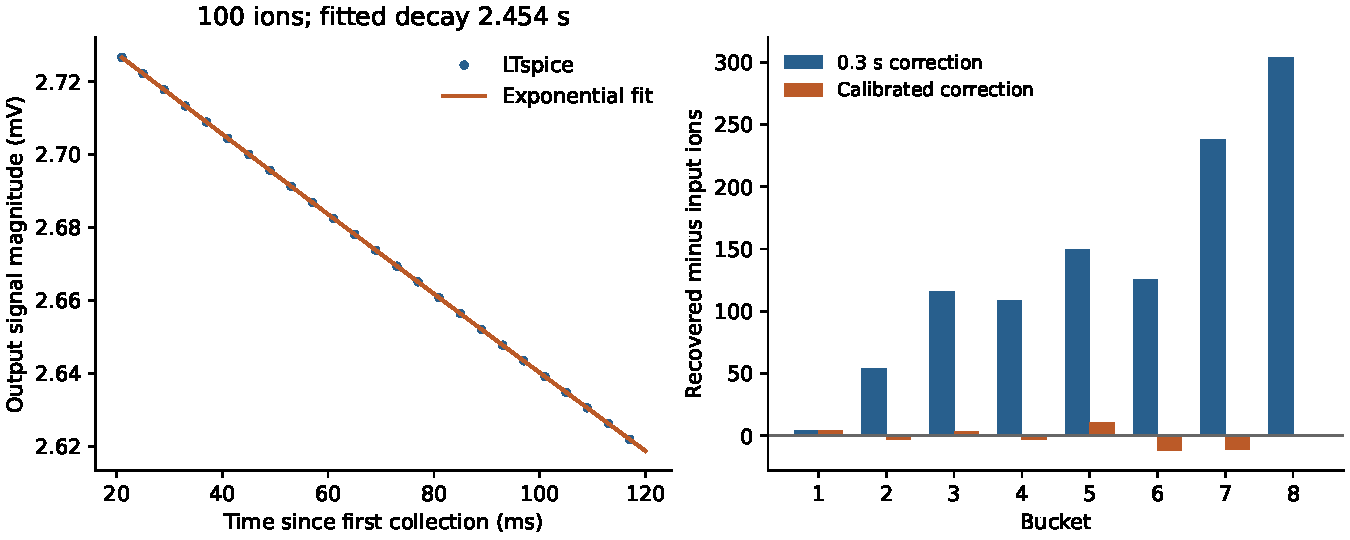
\includegraphics[width=\linewidth]{discharge_calibration.pdf}\end{center}

\section{Validation and reproduction}
The input-bin width and maximum transient timestep are reduced together from
5 to \SI{2.5}{\micro\second}. Integrated input charge is checked against the
finite-path value. Noise calculations compare 200 and 400 spectral points per
decade and quadrature orders 8 and 16. The largest relative change in tested
finite-charge signals is \num{4.03e-06}; the noise-density check changes
RMS noise by \num{7.92e-07}. Both threshold brackets have numerical errors
less than one tenth of their distance from $S/N=5$.

The original 10 and 20 ms studies remain unchanged. Configuration:
\texttt{config/discharge\_calibration.toml}. Inputs, raw and reduced data,
model copies, PWL sources and LTspice logs are stored under
\texttt{results/ltspice/discharge\_calibration/20ms/}.
The scripts record SHA-256 hashes for the configuration, currents, circuit,
model, noise source, simulator and numerical code. Julia performs the physical
calculation; Python acquires LTspice outputs and generates this report from HDF5.
The README gives reproduction commands.
\end{document}
